\documentclass[a4paper, 14pt]{article}

\usepackage[english, russian]{babel}
\usepackage [T2A]{fontenc}
\usepackage [utf8] {inputenc}
\usepackage{amsmath}
\usepackage{indentfirst}
\usepackage{graphicx}

\setlength{\parindent}{1.25cm}
\linespread{1.3}

\title{Разработка программного инструмента для построения стохастических траекторий модели Селькова-Строгаца}
\author{Арцыбашев Г.И., МЕН 300206}
\date{25.12.2022}

\begin{document}
	
	\maketitle
	\newpage
	\tableofcontents
	\newpage
	
	\section{Введение}
		
		
		Данная работа посвящена разработке программы для построения стохастических траекторий модели Селькова-Строгаца.
		
		Рассматриваемая модель описывает колебания в химических реакциях диоксида хлора, иода и малоновой кислоты. Эти колебания носят название гликолиза: распад глюкозы и других сахаров. В 1994 году Строгац предложил динамическую модель, состоящую из двух дифференциальных уравнений для описания динамики реагентов.
	
	
	\section{Описание и анализ модели}
		
		
		Математическая форма записи модели Селькова-Строгаца выглядит следующим образом
		\begin{center}
			\begin{math}
				\begin{cases}
					\dot x = -x + \alpha y + x^2y \\
					\dot y = \beta - \alpha y - x^2y.
				\end{cases} 
			\end{math}
		\end{center}
		
		Здесь переменные $x$ и $y$ "--- концентрации, соответственно, продукта и субстрата, $\alpha$ и $\beta$ "--- положительные кинетические параметры.
		
		Система имеет одну точку покоя с координатами
		\begin{center}
			\begin{math}
				\begin{cases}
					\bar x = \beta, \\
					\bar y = \frac{\beta}{\alpha + \beta^2}
				\end{cases}
			\end{math}
		\end{center}
		
		Здесь и далее мы зафиксируем параметр $\alpha = 0.1$ и будем рассматривать динамику системы в зависимости от параметра $\beta$. Тогда точка покоя $(\bar{x}, \bar{y})$ имеет четыре возможных типа:
		
		\begin{itemize}
			\item $0 < \beta \le 0.161975$ и $\beta \ge 2.381$ "--- устойчивый узел
			\item $0.161975 < \beta < 0.419992$ и $0.789688 < \beta < 2.381$ "--- устойчивый фокус
			\item $\beta = 0.419992$ и $\beta = 0.789688$ "--- центр
			\item $0.419992 < \beta < 0.789688 $ "--- неустойчивый фокус 
		\end{itemize}
		
		\begin{figure}[h]
			\begin{center}
				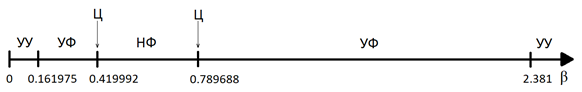
\includegraphics[scale=0.65]{img/type_eq_points.png}\caption{Тип точки покоя в зависимости от параметра $\beta$ (УУ – устойчивый узел, УФ – устойчивый фокус, НФ – неустойчивый фокус, Ц – центр)}
			\end{center}
		\end{figure}
		
		\newpage
		
		В дальнейшем будет рассматриваться следующая стохастическая система
		
		\begin{center}
			\begin{math}
				\begin{cases}
					\dot x = -x + 0.1y + x^2y + \varepsilon\dot{w_1} \\
					\dot y = \beta - 0.1y - x^2y + \varepsilon\dot{w_2},
				\end{cases}
			\end{math}
		\end{center}
		
		где $\varepsilon$ "--- интенсивность случайных возмущений, а $w_1(t)$ и $w_2(t)$ "--- независимые винеровские процессы.
		
	\section{Численный метод решения систем дифференциальных уравнений}
		
		\subsection{Определения}
		
			Прежде чем переходить к компьютерному моделированию стохастических траекторий, необходимо рассмотреть численный метод решения СДУ.
			
			Рассмотрим задачу Коши для системы дифференциальных	уравнений
			
			\begin{center}
				\begin{math}
					\begin{cases}
						\dot x = f(x, y) \\
						\dot y = g(x, y)
					\end{cases}
				\end{math}
			\end{center}
			
			с начальными условиями
			
			\begin{center}
				$x(0) = x_0$
				
				$y(0) = y_0$.
			\end{center}
			
			Пусть пара функций $x(t)$, $y(t)$ является решением этой задачи Коши. Для дискретизации временного отрезка [$t_0, t_0 + T$] разобьем его
			на $N$ частей узлами $t_0 < t_1 < ... < t_N = t_0 + T$ с шагом $h = \frac{T}{N}: t_{m+1} = t_m + h$.
			
			Для дискретизации функций обозначим через $x_m$,  $y_m$ приближенное значение для неизвестного точного решения $x(t_m)$, $y(t_m)$ в момент
			$t_m$. Для расчета $x_m$,  $y_m$ будем использовать метод Рунге — Кутта.
			
		\subsection{Метод Рунге — Кутта четвертого порядка}
			
			Расчет приближенных значений ведется по формулам:
			
			\begin{center}
				$x_{m+1} = x_m + \frac16 \left(K_1 + 2K_2 + 2K_3 + K_4\right)$
				
				$y_{m+1} = y_m + \frac16 \left(L_1 + 2L_2 + 2L_3 + L_4\right)$
				
				$K_1 = hf(x_m, y_m)$, 
				$L_1 = hg(x_m, y_m)$
				
				$K_2 = hf\left(x_m + \frac{K_1}{2}, y_m + \frac{L_1}{2}\right)$, 
				$L_2 = hg\left(x_m + \frac{K_1}{2}, y_m + \frac{L_1}{2}\right)$
				
				$K_3 = hf\left(x_m + \frac{K_2}{2}, y_m + \frac{L_2}{2}\right)$, 
				$L_3 = hg\left(x_m + \frac{K_2}{2}, y_m + \frac{L_2}{2}\right)$
				
				$K_4 = hf\left(x_m + K_3, y_m + L_3\right)$, 
				$L_4 = hg\left(x_m + K_3, y_m + L_3\right)$
			\end{center}
			
			\begin{figure}[!ht]
				\begin{center}
					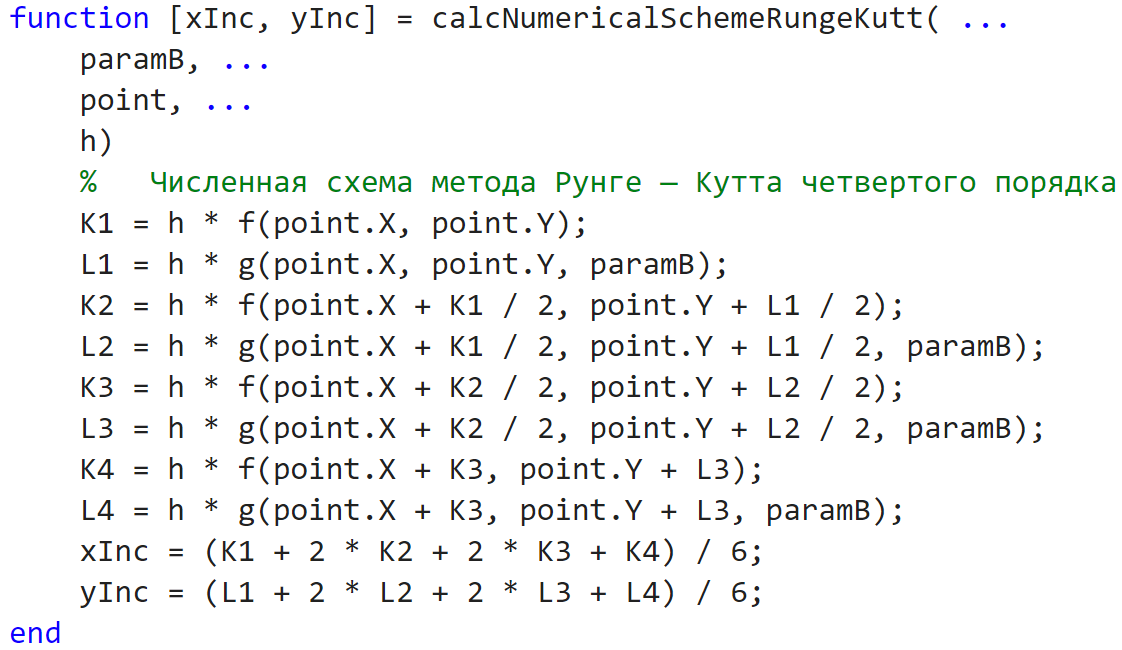
\includegraphics[scale=0.35]{img/codeRK.png}\caption{Код численной схемы метода Рунге — Кутта четвертого порядка}
				\end{center}
			\end{figure}
			
			\begin{figure}[!ht]
				\begin{center}
					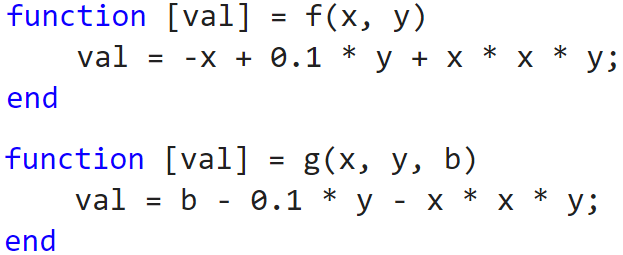
\includegraphics[scale=0.35]{img/code_f_g.png}\caption{Код функций $f$ и $g$, описывающих систему с зафиксированным параметром $\alpha = 0.1$ ($f(x, y) = -x + 0.1 \cdot y + x \cdot x \cdot y$, $g(x, y, \beta) = \beta - 0.1 \cdot y - x \cdot x \cdot y$)}
				\end{center}
			\end{figure}
		
		\newpage
		
	\section{Компьютерное моделирование	стохастических траекторий}
	
		Рассмотрим систему со случайными возмущениями
		
		\begin{center}
			\begin{math}
				\begin{cases}
					\dot x = f(x, y) + \varepsilon\dot{w_1} \\
					\dot y = g(x, y) + \varepsilon\dot{w_2},
				\end{cases}
			\end{math}
		\end{center}
		
		где $\varepsilon$ "--- интенсивность случайных возмущений, а $w_1(t)$ и $w_2(t)$ "--- независимые винеровские процессы.
		
		Расчет приближенных значений на основе метода Рунге — Кутта четвертого порядка ведется по формулам
		
		\begin{center}
			$x_{m+1} = x_m + \frac16 \left(K_1 + 2K_2 + 2K_3 + K_4\right) + \varepsilon\Delta{w_{1, m}}$
			
			$y_{m+1} = y_m + \frac16 \left(L_1 + 2L_2 + 2L_3 + L_4\right) + \varepsilon\Delta{w_{2, m}}$,
		\end{center}
		
		где $\Delta{w_{1, m}}$, $\Delta{w_{2, m}}$ "--- приращения винеровских процессов "--- можно	получить по формулам
		
		\begin{center}
			$\Delta{w_{1, m}} = \sqrt{-2h\ln (r_{1, m})} \sin (2\pi r_{2, m})$
			
			$\Delta{w_{2, m}} = \sqrt{-2h\ln (r_{1, m})} \cos (2\pi r_{2, m})$,
		\end{center}
		
		где $r_{1, m}, r_{2, m}$ "--- независимые случайные величины, равномерно распределенные на отрезке [$0, 1$].
		
		\begin{figure}[!ht]
			\begin{center}
				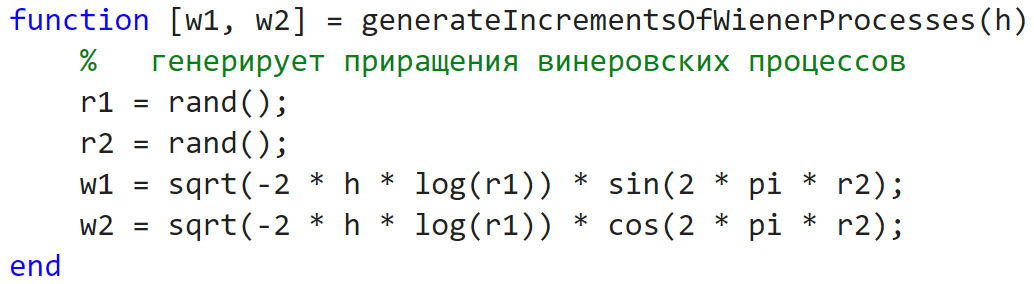
\includegraphics[scale=0.35]{img/code_wiener.png}\caption{Код функции, генерирующей приращения винеровских процессов}
			\end{center}
		\end{figure}
		
		\newpage
		
		\begin{figure}[!ht]
			\begin{center}
				\includegraphics[scale=0.35]{img/code_St.png}\caption{Код функции, генерирующей точки графика стохастической траектории}
			\end{center}
		\end{figure}
		
	
	\section{Работа с программой}
	
		\subsection{Интерфейс}
			
			Интерфейс программы позволяет задавать следующие входные параметры:
			
			\begin{itemize}
				\item параметр $\beta$
				\item количество точек в траектории
				\item шаг численной схемы Рунге "--- Кутта
				\item интенсивность шума
				\item стартовую точку
			\end{itemize}
			
			При нажатии кнопки "Построить" программа по входным параметрам строит стохастическую траекторию	модели Селькова-Строгаца при $\alpha = 0.1$.
			
			\begin{figure}[!ht]
				\begin{center}
					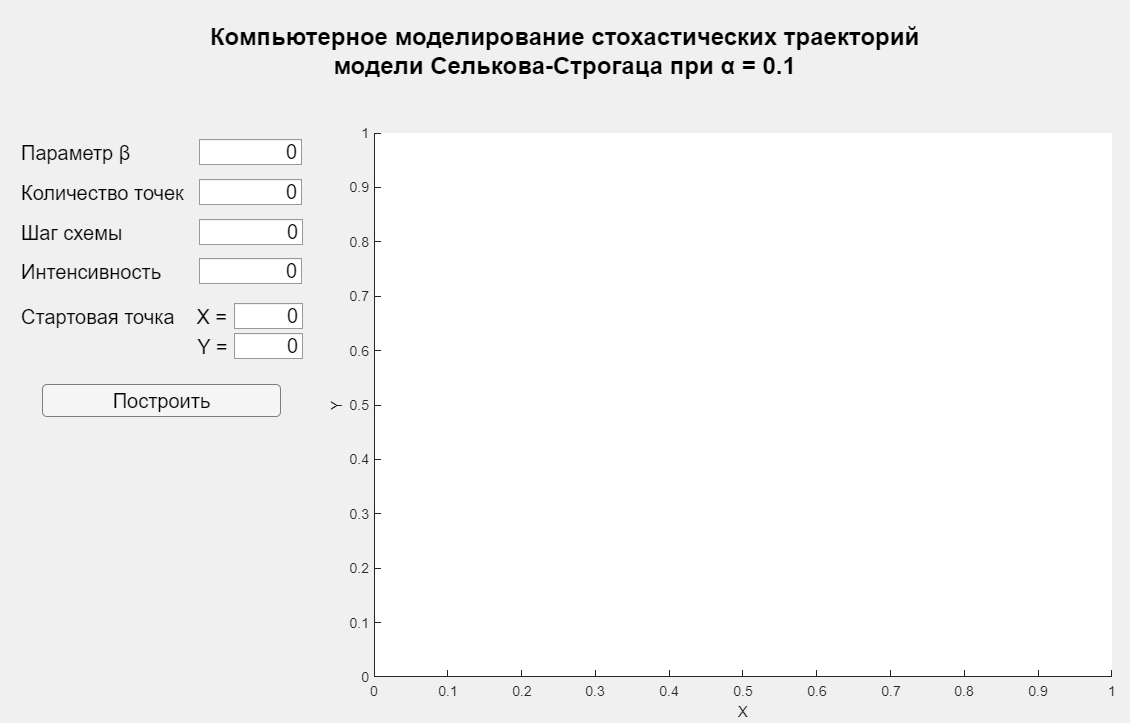
\includegraphics[scale=0.35]{img/interface.png}\caption{Интерфейс программы}
				\end{center}
			\end{figure}
						
			\begin{figure}[!ht]
				\begin{center}
					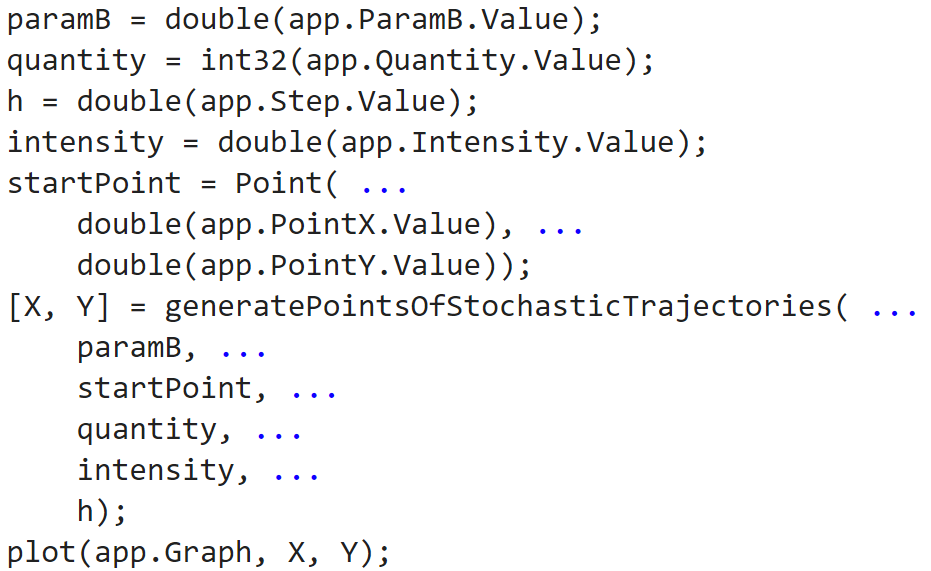
\includegraphics[scale=0.35]{img/callback.png}\caption{Код, выполняющийся при нажатии кнопки "Построить"}
				\end{center}
			\end{figure}
		
		\newpage		
		
		\subsection{Примеры работы программы}
		
			\begin{figure}[!ht]
				\begin{center}
					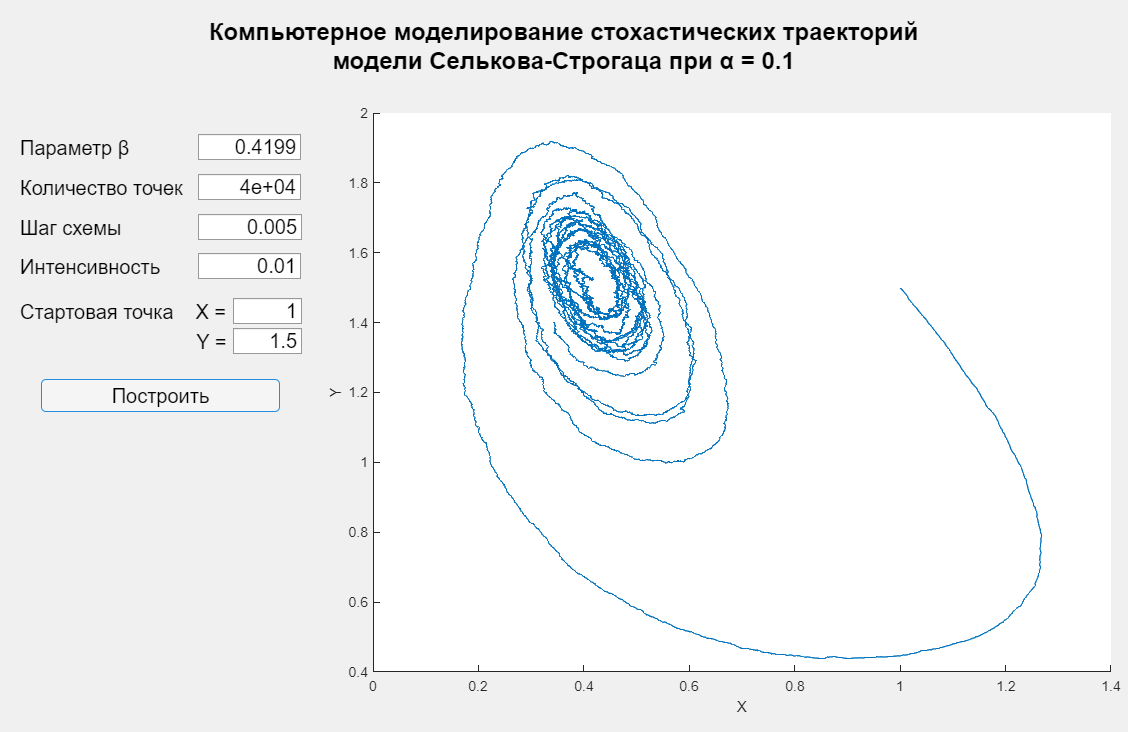
\includegraphics[scale=0.35]{img/ex1.png}\caption{Пример работы программы}
				\end{center}
			\end{figure}
		
			\newpage
			
			\begin{figure}[!ht]
				\begin{center}
					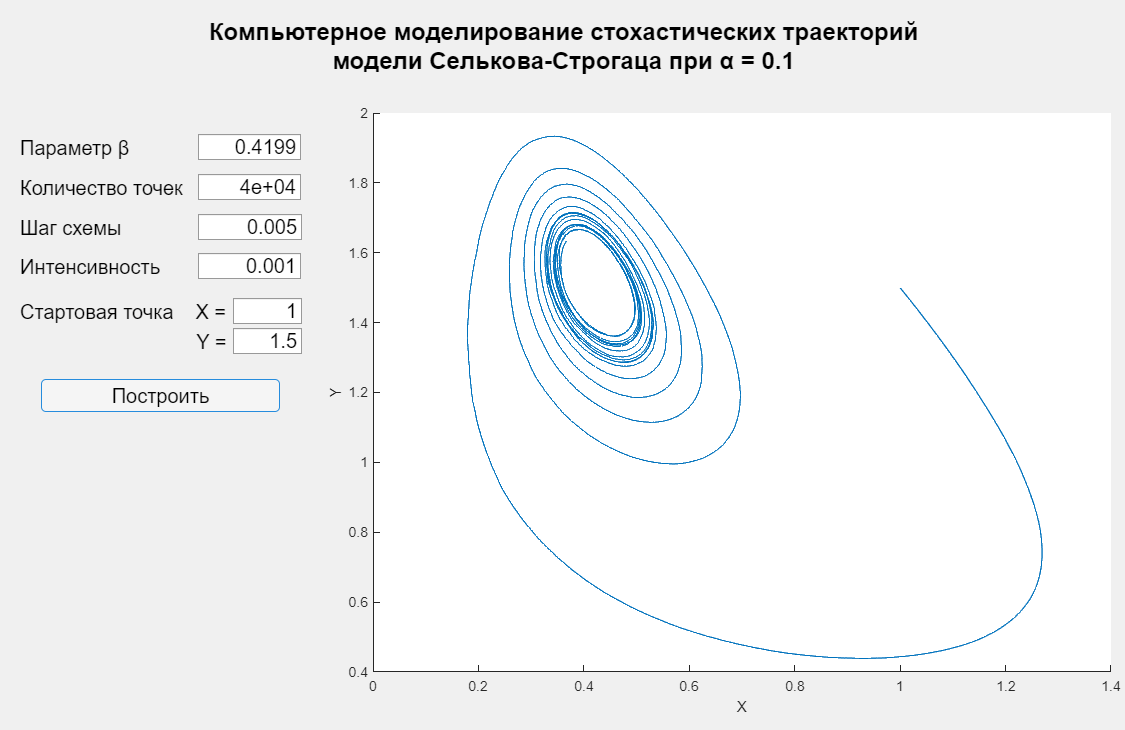
\includegraphics[scale=0.35]{img/ex2.png}\caption{Пример работы программы}
				\end{center}
			\end{figure}
			
			\begin{figure}[!ht]
				\begin{center}
					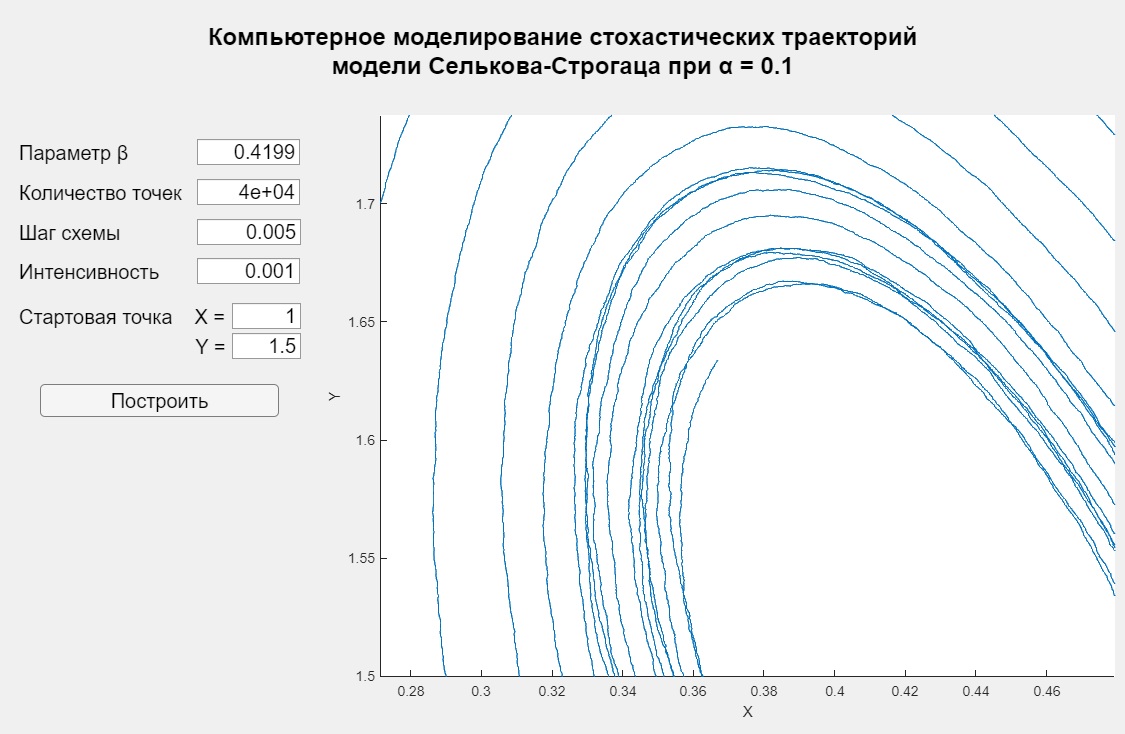
\includegraphics[scale=0.35]{img/ex3.png}\caption{Пример работы программы}
				\end{center}
			\end{figure}
		
			\newpage
			
			\begin{figure}[!ht]
				\begin{center}
					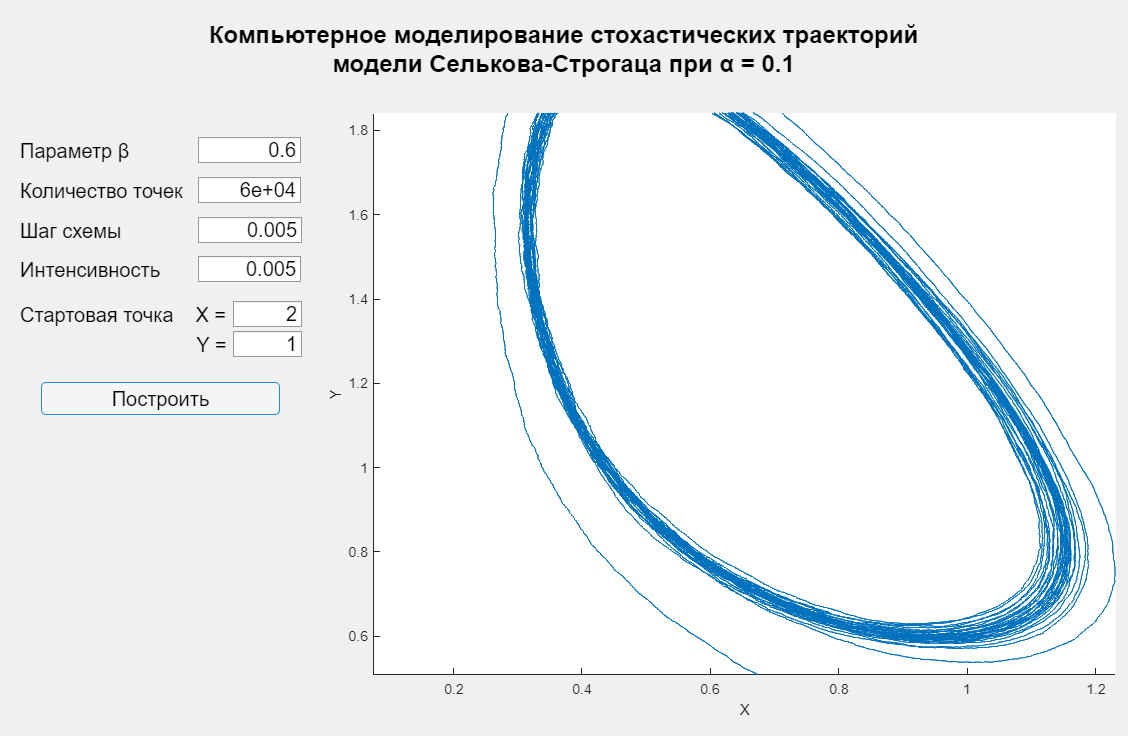
\includegraphics[scale=0.35]{img/ex4.png}\caption{Пример работы программы}
				\end{center}
			\end{figure}
		
		\newpage
	
	\section{Заключение}
		
		Результатом выполнения работы является работающая программа, выполненная в среде MATLAB, позволяющая строить стохастические траектории модели Селькова-Строгаца. Дальнейшим развитием работы может быть улучшение данной программы (например, обработка некорректного ввода входных параметров).
		
\end{document}